\chapter{Background}
\section{Handover}
Handover is when an active cell connection (data or cellular) is transferred from a source base station to a target base station to maintain continuous connectivity for mobile devices. Handover is a crucial technique in radio communication networks for mobility management and load balancing.

A UE \footnote{User Equipment - any device that can connect to a cell network, for instance, a mobile phone} will have an active connection to a single base station (BS) at one time, with its signal strength being measured by the UE in terms of its Received Signal Reference Power (RSRP), which is used in handover triggering. RSRP can be affected by several different factors. Still, the two main influences are the distance to the base station (as propagation loss is logarithmically proportional to distance) and line of sight (LOS) blockages (as direct waves have higher power than reflected waves). 
RSRP is correlated with data throughput, and we want to maximise RSRP to maximise quality of services (QoS). A cell connection will also become unstable or drop at low RSRP strength.

\subsection{Handover Procedure}
\begin{enumerate}
    \item A UE will measure the RSRP of all BSs in range and send the report to the connected (source) BS.
    \item The source BS will compare the measured RSRP metrics and decide whether to initiate a handover. This decision is made with various algorithms discussed in \ref{sec:algorithms}, but all focus on maximising the UE's QoS by handing the connection over to a BS with a higher RSRP (or RSRQ).
    \item If the BS initiates handover, it will determine which neighbouring BS to transfer the connection to. Various protocols determine how a connection is transferred; however, this is outside this paper's scope. Regardless of the protocol used, there will be a drop in connectivity and throughput.
    \item The connection between a UE and the source BS can drop if the handover is not triggered before the RSRP drops below a level where communication is possible. This is termed handover failure (HOF), which has a much greater impact on connectivity, so the frequency of these failures must be minimised.
    \item Handover decisions are not always optimal; a UE transferred to a neighbouring BS could be transferred back to the source BS if the RSRP values are unstable. This results in two unneeded handovers, decreasing QoS and increasing server load. This is termed Handover Ping Pong (HOPP), as it must be minimised.
\end{enumerate}

\subsection{Indoor Environments}
The challenge of handover is relatively simple in outdoor environments, and with it being the main target of literature on the subject, many solutions exist to its various challenges. 5G, however, will be ubiquitously deployed in indoor environments. The indoor wireless channel is much harder to model, as LOS blockages are much more common due to the constrained environment. Furthermore, indoor deployments lend themselves towards much smaller cells (the area a BS serves); therefore, handovers will occur much more frequently in these high-density deployments.

Therefore, this paper's primary motivation and focus is on understanding, modelling, and predicting handover in indoor environments to maintain a high level of connection quality.

\section{Handover Algorithms}
\label{sec:algorithms}
This paper focuses on understanding the effects of handover and designing and testing various strategies to minimise the adverse effects. We, therefore, need to understand the different methods used to initiate handover and classify the multiple algorithms.

\subsection{Classical Approach}

\begin{wrapfigure}[18]{r}{0.5\textwidth}
    % \centering
     \raisebox{0pt}[\dimexpr\height-2\baselineskip\relax]{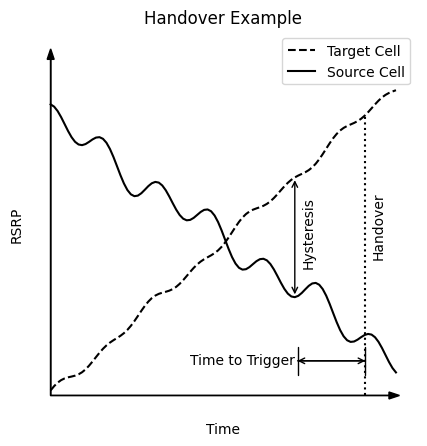
\includegraphics[width=0.48\textwidth]{src/img/hysteresis_ttt.png}}
    % 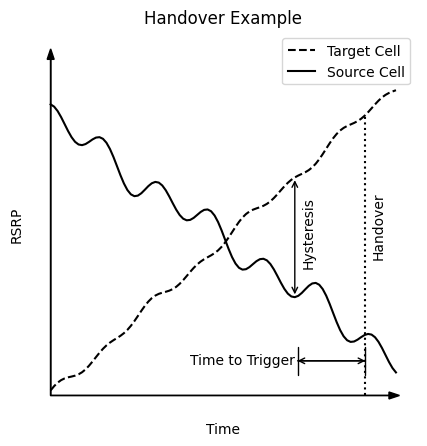
\includegraphics[width=0.48\textwidth]{src/img/hysteresis_ttt.png}
    \caption{handover based on Hysteresis and TTT}
    \label{fig:hysteresis_handover}
\end{wrapfigure}

The standard approach towards handover uses two parameters, \textit{Hysteresis} and \textit{Time to Trigger}, to determine when to trigger handover. When a neighbour cell has an RSRP greater than the current cell by a set margin, i.e. the Hysteresis, for a given period, i.e. time to trigger, the handover is triggered, and the UE is transferred to the neighbour cell. This process is illustrated in Figure \ref{fig:hysteresis_handover}. Alternative heuristics are often needed, as the standard approach is not robust enough for dynamic environments.



\clearpage %============================= CLEAR PAGE  =====================================%

\subsection{Alternative Heuristics}
Most existing handover algorithms use relative RSRPs (such as Hysteresis) with some delay (such as Time to Trigger). The literature suggests and models other parameters, including throughput, UE location, load balancing, user velocity, service delay, and distance. \cite{nyangaresi_efficient_2022}.

\citet{hatipoglu_handover-based_2020} presented a handover-based load balancing algorithm for HetNets. The paper utilised UE speeds in determining handover, which is an unrealistic metric to obtain in practice. The algorithm itself is pretty simplistic, and while the paper showed promising results, the algorithm does not consider critical metrics such as RSRP or connection speed.

\subsection{Machine Learning}
Seeing handover as an optimization problem, using machine learning (ML) to solve it is natural. ML techniques are appealing because they offer potential performance improvements in complex domains where heuristic approaches struggle. As ML techniques do not require a model of the environment, this is especially applicable to indoor environments, where modelling proves difficult.

ML algorithms can be subdivided into supervised, unsupervised and reinforcement learning. Supervised and unsupervised algorithms perform regression or classification on a set of inputs. Reinforcement learning is based on the idea that the algorithm will learn to maximise its rewards in a given environment by learning the optimal policy. In our case, the optimal policy is a sequence of handover decisions that maximise throughput while minimising HOF and HOPP. The use of reinforcement learning has been surveyed in \cite{mollel_survey_2021}.

Reinforcement learning is a broad grouping of algorithms. These include Multi-Armed Bandits, Monte Carlo methods, and Deep Q-learning.

\citet{yajnanarayana_5g_2020} presented a handover algorithm using Contextual Multi-Armed Bandit reinforcement learning. This ML model provided modest improvements (0.3dB) in the average RSRP of devices. The authors also built their custom network simulator, which used sophisticated propagation models like log-shadowing and the WINNER UMa Model. The code used to simulate it was not released, providing very little reproducibility of the paper. The improvements were relatively minor, and better results could be obtained with a deep-learning-based Reinforcement model.

\citet{mollel_survey_2021} further introduces and surveys an alternative machine learning method. The pure network-based models operate only on radio data, such as RSRP and base station states. However, an alternative heuristic uses optical information, such as camera feeds, to predict handover better. This is done by tracking UE movement through object detection and predicting when LOS will be obstructed. While this tool can prove very useful, it introduces many limitations, as the models trained will be very location-dependent and have the most significant impact in indoor environments due to the greater LOS blockage rate.

\section{Handover Testbeds}
To evaluate experimental algorithms, we need some way to emulate a network. Many authors run custom simulations using propagation algorithms to model path loss and simulate the network devices. A better method is using a software radio suite as a testbed. This allows us to emulate UEs, base stations (BSs), and the core network (CN).

A few options are available, with the significant software being srsRAN, OpenAirInterface, and Aether. This paper chose srsRAN due to its clear open-source code and extensive tutorials. While a fully custom testbed allows for greater flexibility, the realistic nature of using software radio suites will give results that much better reflect how the algorithms would perform in a real-world scenario and, so, arguably, provide more useful results.

\citet{powell_handover_2021} presented a testing framework for 4G experiments using srsRAN and performed basic experiments. The framework was presented clearly, and we were able to replicate the results of their simulation. The experiments they performed, however, were limited as signal strength was arbitrarily introduced by attenuating a signal and did not utilise signal propagation algorithms.

\section{Previous Work}

\citet{sucasas_simulation_2019} explores the effect of cell size on various handover metrics, such as HOPP and HOF. This paper tackles handover in ultra-small cell deployments, which have similarities to indoor settings. The paper's results show a highly significant increase in ping-pong rates and HOF for cells with a smaller than 200m Inter-Site Distance (ISD) - the distance between two eNBs- leading us to conclude similar problems in our indoor scenario. However, the results were achieved through simulation, which does not account for the various secondary effects of indoor scenarios mentioned above.

\citet{bertolini_evaluating_2021} presents a real-world experimental setup using OpenAirInterface and conducts various experiments to understand handover impact. However, this paper does not translate well to our domain, as physical cabling connects to each cell instead of a radio transceiver. This limits the results of their experiment, as no second-order effects are seen (LOS blockage, signal reflection and open-air propagation loss). The paper also outlines the handover protocol in an easy-to-understand way, which aids us in our understanding. This paper finds both a constant latency penalty in handover experiments and a drop in throughput when handover occurs.

\citet{zhang_performance_2012} presents an in-depth study on the impact of handover on TCP and UDP traffic. Their experiments used a similar cabled setup as \citep{bertolini_evaluating_2021} for their first experiments but used an outdoor testbed for the latter. The paper found a clear relationship between the hysteresis value and HO rate; however, it found no impact on TCP traffic. It further measured the latency introduced by a handover to be 80ms, a value we reproduce in Section \ref{sec:handover-impact}.

\section{Further Technologies}
When examining the directions for this paper, three possible technologies should be reviewed as they strongly relate to either handover performance or experimentation. 

\subsection{Reactive vs Predictive Handover}
There are two main strategies when dealing with handover. We can either react to degraded quality and handover to improve it, or we can predict when quality is about to degrade and handover to maintain the quality of the connection.

\subsubsection*{Reactive Handover} This is the traditional handover mechanism where the decision to switch a UE from one eNB to another is made based on the current signal strength and quality. This relies on a more static environment where no sudden drops in signal connection occur; if a connection falls below a certain threshold, the UE cannot communicate the degraded connection to the eNB base station and must perform a reconnection to the network -- which incurs a more significant penalty. This also relies on real-time signal metrics, as a delayed response to a falling signal strength could result in an HOF. While drawbacks exist when there is not a long enough window to react, it is a much simpler algorithm to implement. It is chosen for most outdoor handover scenarios, with a notable exception in high-speed movement applications such as railways \cite{kosmopoulos_handover_2022} and other dynamic environments.
                
\subsubsection*{Predictive Handover} Predictive handover instead attempts to predict when signal quality is about to drop and initiates handover before the signal quality drops below a certain threshold. It aims to minimize disruption and enhance the user experience by anticipating network conditions \cite{al-quraan_enhancing_2023}. This avoids HOF, as seen in reactive handovers, but relies on accurate predictions. Prediction misses could instead lead to more unnecessary handovers, some of which may be classified as Ping Pong Handovers. Many predictive handovers utilise UE movement speed to estimate when to initiate a handover. However, many now leverage machine learning algorithms to predict the need for handover. This requires accurate historical data and real-time analysis for prediction, and signal processing techniques are incorporated to analyze patterns and predict future signal degradation.

% \textcolor{orange}{I think the paragraph below needs to be on the discussion. This section is to provide what is needed to understand handover and related works. }

% \subsubsection*{This Paper} While we aim to examine the performance of reactive handovers in indoor environments initially, we wish to examine the feasibility of introducing a Predictive Handover algorithm. However, this may be beyond this paper's scope, so we instead lay the groundwork for future research in this area. 

\subsection{Large Scale Emulators}
We can fully simulate network environments in software; however, this is limited in its ability to extract valuable insights for new environments. There is an alternative, however, in the form of large-scale network emulators, the largest of which are the Platforms for Advanced Wireless Research (PAWR). These do not rely on software simulation but consist of real-world software-defined radio testbeds. Specifically, their POWDER platform is a city-wide testbed in Utah, United States. 

POWDER allows researchers to run experiments without maintaining and deploying networks themselves. This removes many barriers to entry in the research of 4G/5G networks, as equipment costs can be high. It also enables researchers to test machine learning models for predictive handover and assess signal processing algorithms in a controlled environment \cite{rusca_mobile_2023}.

For this paper, POWDER was not used as the group already had a working testbed; however, this remains a viable route for larger-scale experiments for an extension to this project. However, the drawback is the inability to perform mobility experiments, as radio attenuation is software-defined. This inherently limits us from performing our indoor experiments, where open-air radio propagation is what we are interested in.

\subsection{O-RAN}
Open Radio Access Network (O-RAN) architecture is a new software standard for interoperability and flexibility in 5G networks. It defines standardised interfaces (E2) for modular radio network components to communicate over and includes the RAN Intelligent Controller (RIC), a software-defined component responsible for controlling and optimising RAN functions \citep{juniper_networks_uki_what_2022}. 

This enables the integration of machine learning directly into the radio access network for smarter handover decisions and innovation and customization in handover strategies by allowing third-party applications and services within the RAN  \cite{niknam_intelligent_2020}. 

% possible additions: CQI, hard/soft handover, S1/X2 handover
% 6 pages, need to expand to maybe 7?

